%!TEX root=report.tex
\subsection{KMeans}
First off what needed to be identified was the number of clusters. 
Due to the size of the design matrix $X$, (64800,341), and the fact multiple simulated datasets of the same size would be needed to calculate the gap-statistic it was decided to leverage the high performance computing (HPC\footnote{link: http://www.cc.dtu.dk/}) cluster that DTU offers for students and faculty. 
 It should be noted that if such a setup was not available one could have used smaller samples and/or a variant of KMeans using so called "minibatches". \\
5 simulation samples of size (64800,341) was made using a multivariate uniform distribution. The following is the plot of the resulting gap statistic $\pm$ the standard deviation:
\begin{figure}[H]
	\center
	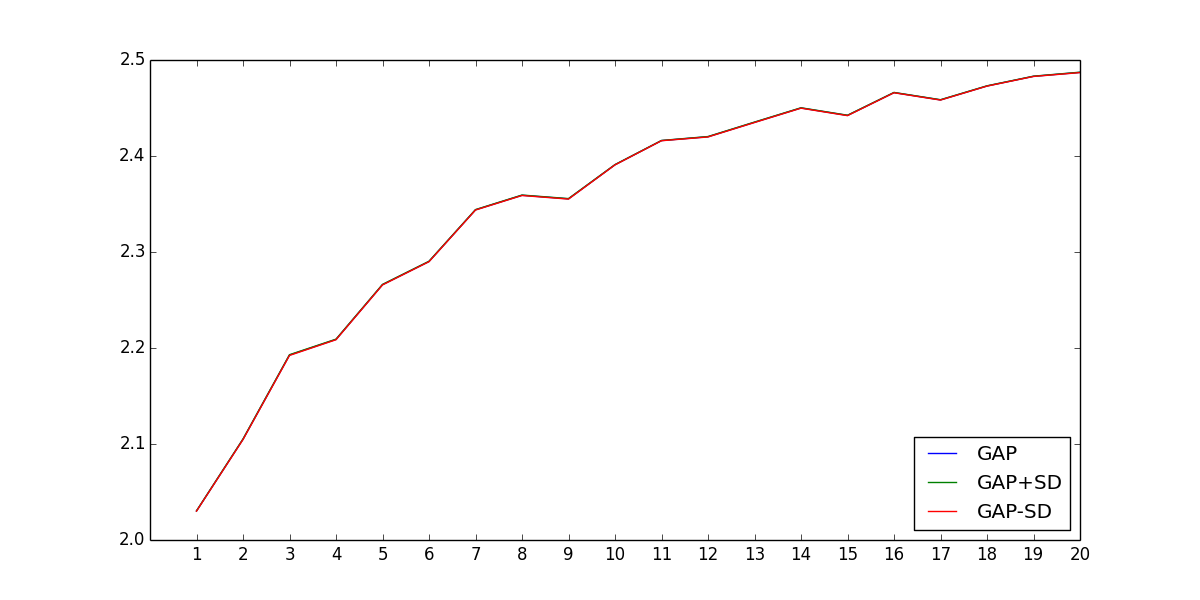
\includegraphics[width=\textwidth]{figures/gap.png}
	\caption{Gap statics and standard deviation. It is not an error that the 3 lines overlap; it is simply caused by the large amount of simulation samples which leads to a very small $W_k$ which in turn causes $SD(Log(W_k)$ to be small ($\approx 10^{-3}$)}
	\label{fig:gap}
\end{figure}

So based on the gap statics plot (or by writing a loop to iterate through values until $gap(k)\ge gap(k+1)-sd(k+1)$) one obtains that 8 clusters should be used